\chapter{Discussion}
This chapter is dealing with the observed results.

\section{Results}
Looking at \autoref{fig:coverages} it is visible that the projects of the lowest quantile do not change concerning the coverage of the regions automatically optimizable by Polly.
So about 25\% of the programs would not have any profits when extending all of their \scops the next surrounding region.
Investigating the upper two parts of the plots shows that there are at least some projects which would have benefits if they were extended.
That the projects in the lowest quantile remain almost with the same coverage and the projects of the upper two quantiles slightly move up is also becoming manifest in looking at the increment of the variance and the standard deviation in \autoref{tab:statsMatrix}.\\
Nevertheless there are some regions classified as unprofitable which would have great impacts to the coverage.
\Eg in the function send\_bits(...) within the file bits.c of the project bzip2 there is a \scop with a duration of about \(12864 \mu s\) but its parent has a duration of \(9409596 \mu s\) which is about 750 times bigger.
\begin{comment}
    \autoref{fig:fatParent} shows a region within the project bzip2 which is really tiny (A red arrow is pointing on that region with green background) but its parent represents the hole function.
    The parent was rejected because the parent is a toplevel region due it contains the hole function.
    \begin{figure}
        \caption[A region tree of bzip2]{
            A region tree of the method \texttt{mainSort} within the file blocksort.c of the project bzip2.
            The red arrow points to a region which is very tiny but its parent contains the hole function.
            So there is hugh difference between the duration of the region and its parent.
        }
        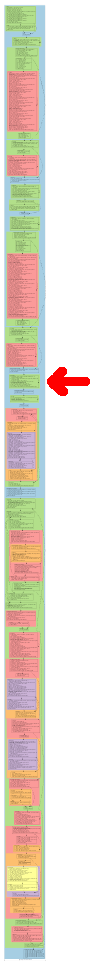
\includegraphics[height=\textheight]{gfx/fatParent.png}
        \label{fig:fatParent}
    \end{figure}
\end{comment}
But not all of the \scops can be simply extended.
\Eg the regions rejected because they are top level regions can not be extended until they are put into a larger context -- this means inlining.
Also regions rejected because of uncomputable loop bounds can only get valid if their loop bounds can be computed \eg by performing \jit compilation.
Reasons for rejecting like \enquote{Non affine access function}, \enquote{Non affine branch in BB} and \enquote{Non affine loop bound} (where the loop bound could be computed) can only be eliminated if they are transformed to an affine linear version or practical methods for handling non-affine expression are found.
But this is not possible in general or at least not practical (see \autoref{sec:altExt}).
Also the part stating that Polly did not return a reason for rejection is currently not likely to be optimizable because the exact reason for rejection is not known.

\section{Threads to Validity}
\subsection{Construct Validity}
The overhead of executing additional instructions for taking measurements is investigated and graded as negligible because it takes about \measurementOverhead to execute an enter and an exit call \overheadIterations times averaged over \overheadRounds rounds.
Also when parents of \scops which are measured are also measured the entry and exit call of the inner measurement causes a slight increase of the duration of the outer measurement.
This is also negligible due to the same reason.
The program used for checking this is attached in \autoref{lst:checkOverhead}.\\
For minimizing the influences of saving the data collected on run time it is only written to the database once at the very end of the executed project.\\
\subsection{Internal Validity}
The measurements are rely on the quality of the input data brought by benchbuild.
This problem is addressed by benchbuild in relying on benchmarks which are included by the projects or benchmarks like SPEC2006 which are accepted by the community.
This does not mean the dependence of the results to the input is vanishing.
But it can be assumed that the test cases cover the most important and most common use cases.
\subsection{External Validity}
The selection of subject programs threatens the generalizability of the results but is controlled by selecting a large and diverse number of programs randomly.
